% Chapter Template

\chapter{Literature overview} 

\label{Chapter3} % Change X to a consecutive number; for referencing this chapter elsewhere, use \ref{ChapterX}

%\lhead{Chapter 3. \emph{Literature overview}} % Change X to a consecutive number; this is for the header on each page - perhaps a shortened title

%----------------------------------------------------------------------------------------
%	SEGMENTATION
%----------------------------------------------------------------------------------------

\section{Cell segmentation}

Several studies have been proposed to classify autoantibody fluorescence patterns by using an automatic thresholding method, i.e.  Otsu's method, to segment the cells. The  thresholding method can choose the threshold to minimize the intraclass variance of the black and white pixels automatically. Due to the variety of ANA patterns,  Otsu's algorithm always failed to segment cells of speckled and nucleolar patterns, such as cases of a very blury image of low intensity. Figure \ref{fig:BadSegment} shows the over-segmentation results by using Otsu's algorithm. Additional challenge for the segmentation here is to separate overlapping cells which are quite common in the process.

\begin{figure}[htbp]
	\centering
	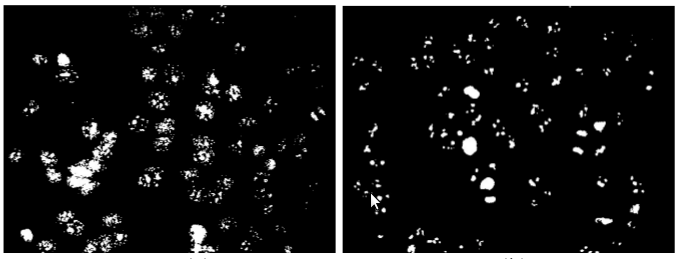
\includegraphics[scale=0.4]{Figures/introduction/badsegmentation}
	\rule{35em}{0.5pt}
	\caption[Bad segmentation example]{Segmentation results of the Otsu method (from \cite{Huang2008})}
	\label{fig:BadSegment}

\end{figure}


In \cite{Huang2008}, Huang et all. present an adaptive edged-based segmentation method for automatically detecting outlines of fluorescence cells in IIF images. Their approach is based on specific properties of the images regarding the pattern class. They have divided the images in two groups : sparse region and mass region cells. The mass region cells are those ones which have a \textit{compact} appearance, that look like a smooth object, while the sparse region cells are those ones for which we can detect multiple object in a cell. The approach trains a classifier to classify each image in the groups and applies different segmentation procedure for each group. In the case of the mass region cells, the cells are segmented using Otsu segmentation method, while in the case of the sparse region cell segmentation is performed by an edge detection. Their approach resulted in better segmentation results, but approximately 10\% of the cells remained undetected.

In \cite{HuangWatershed}, same authors further improve their method by incorporating watershed segmentation. The second approach also includes segmentation in two stages, depending on defined criteria. After a segmentation step performed by the watershed, the approach merges parts located relatively close and eliminates parts not large enough to represent a cell. If the retrieved number of regions doesn't safisfy the defined criteria, the segmentation step is performed again with different parameter settings determinated by Otsu's thresholding. 

All forementioned approaches report similar shortcomings : approximately 10\% of cells remained undetected and the inability to separate overlapping cells.  The focus of the segmentation part of the Thesis will be on overcoming those problems.



%-----------------------------------------------------------------------------------------
%   INTENSITY LEVEL CLASSIFICATION
%-----------------------------------------------------------------------------------------

\section{Intesity level classification}

The following step, the intensity level classification, hasn't attracted a lot of scientific research, but has demonstrated remarkable results so far.

In \cite{SodaIntensity2006},  authors propose a system based on  \textit{Multi-Layer Perceptrons} and a \textit{Radial Basis Network} for the intensity classification step. That system, which makes use of features inspired from medical practice, shows error rates  up to 1\%, but it uses a reject option and it does not cast a result in about 50\% of cases. In \cite{SodaIntensity2009} the authors further refine their system. They train three experts, one specialized for each class, with a different set of features. They threat the classifiers similar to the \textit{one-vs-all} approach, so the final decision is made by a classifier most certain in it's decision. The authors report a success rate of 92,6\% accuracy.


%-----------------------------------------------------------------------------------------
%   STAINING PATTERN CLASSIFICATION
%-----------------------------------------------------------------------------------------

\section{Staining pattern classification}

As this problem was emphasized on the \textit{International Conference on Pattern Recognition 2012} as a contest, this step has been well researched and several very successful methods have been proposed. In \cite{FoggiaBenchmarks2013}, Foggia et al. provides a detailed overview of the methods submitted for the contest. The three most successful ones are presented here. 

In \cite{Kuan2012}, Kuan presents a method based on four texture descriptors: a rotation invariant form of local binary patterns (LBP) with multi-scale analysis,discrete cosine transformation, the mean values and standard variances of 2-D Gabor wavelets, and some global appearance based statistical features. A multiclass SVM was trained on each class of the four feature sets. The SVMs are then integrated in one classifier by using the AdaBoost.M1 algorithm.

In \cite{Nosaka2012}, Nosaka presents a similar approach on an extension of LBP, namely CoALBP \cite{Nosaka2011}. The advantage of this method is that the method can observe not only locals LBP, but also the spatial relations among adjacent LBP. The classifier is a linear SVM trained on an extended dataset including the rotated patterns of the original images. 

Xianfeng et al. proposed a system based on MR8 method \cite{Varma2005} to extract statistical intensity features. The method calculates filter responses locally on the image, and then trains a global texton dictionary using $K$-means clustering. In that way, each image is represented by the frequency histogram of textons. The decision is made by a $k$-NN classifier.

Although there are many more papers in existance covering this problem, they are not presented here due to different, and not so rigorous, evaluation. Most of the early work was done on private datasets not available to public, which makes them not comparable to the new research results. Other papers with  a more recent date do not follow the evaluation procedure, so it is very hard to compare their efficiency with those ones in the overview. 

More recently, a new overview of the method was presented by Agrawal et al. in \cite{Agrawal2013}. The committee of \textit{ICPR'13} has released a new, much bigger dataset for the same problem. The authors experimented with the most commonly used features in the previous contest - statistical features, histograms of oriented gradients, shape and size descriptors and texture descriptors. They have chosen the most typical representatives of classifiers, namely Naive Bayes, k-NN, SVM and Random forest. The SVM with Law's textural representation significantly  outperformed other classifiers and feature representations.


